% Apuntes sobre el paquete beamer: http://metodos.fam.cie.uva.es/~latex/apuntes/apuntes.html (Universidad de Valladolid)
\documentclass{beamer}

\usepackage[utf8x, utf8]{inputenc}
\usepackage{ucs}
\usepackage[T1]{fontenc}
\usepackage{lmodern}
\usepackage[spanish]{babel}
\usepackage{graphicx}
\usepackage{tabu}


\newcommand{\software}{\textit{software }}

% Configuración de Beamer
\mode<presentation>{\usetheme{Berkeley} \setbeamercovered{dynamic}}
% Otros temas semejantes: Madrid, PaloAlto, Ilmenau, Berkeley, Rochester
\logo{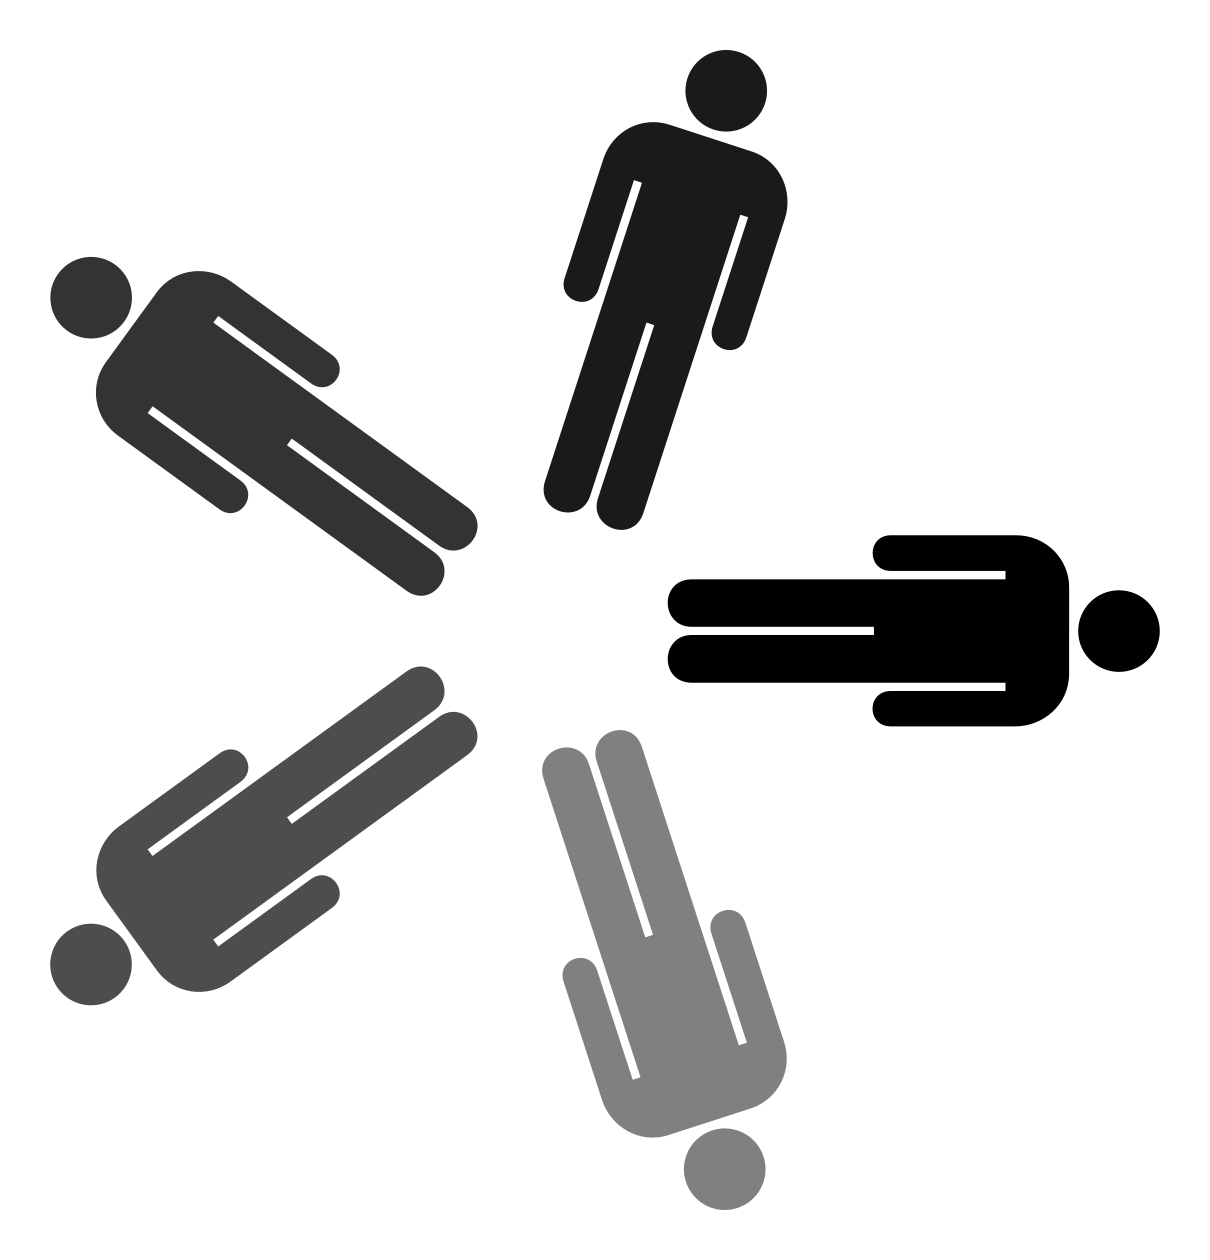
\includegraphics[scale=.04]{logodiedral.pdf}}
\institute{Universidad Complutense de Madrid}

\title[ACE]{\itshape Airline Common Environment}
\author{Grupo $\mathcal{D}$iedral}
\date{20 de diciembre de 2012}

\begin{document}
\maketitle

	\frame{\frametitle{Resumen} \tableofcontents}
	
	\section{Introducción}
	
\begin{frame}
	\frametitle{Descripción general}
	
	\begin{block}{Resumen}
		\textit{Airline Common Environment} es un producto \software destinado a la gestión integral de una compañía aérea.		\end{block}

	\begin{itemize}
		\item Propósito y alcance
			\begin{itemize}
				\item Gestión interna
				\item Gestión externa
			\end{itemize}
		\item Perspectivas y funciones del producto
		\item Características del usuario
		\item Restricciones y dependencias
	\end{itemize}
\end{frame}

\begin{frame}
	\frametitle{Estimación}

	\begin{block}{Cálculo de los puntos de función} \centering \scriptsize
	\vspace*{2mm}
	\begin{tabu} to .9\linewidth { X[6, l]  X[1, r] }
		Gestión corriente de la base de datos \dotfill & 152\\
		Configuración de la base de datos \dotfill & 50\\
		Interfaz externa \dotfill & 51\\
		Interfaz interna \dotfill & 113\\
		Generación de gráficas \dotfill & 14\\
		Análisis y monitorización de datos \dotfill & 47\\
		\multicolumn{1}{r}{Total} & 427 \\
	\end{tabu}
	\vspace*{2mm}
	\end{block}

	\pause

	\begin{block}{Resultados}
		\begin{itemize}
			\item $\mathrm{PFA} = \mathrm{PFSA} (0,65 + 0,01 \cdot \mathrm{FCT}) = 465,43$.
			\item 30.718,38 líneas de código en C++.
			\item COCOMO: 279,2 hombres/mes y 22.631 LOC en Java.
		\end{itemize}
		
	\end{block}
\end{frame}

\end{document}
